\chapter{PROBLEM}
\section{Problem Definition}
The basic problem in this thesis is how to find appropriate job descriptions by user's r\'esum\'e, which means we need calculate the similarity between the user��s r��sum�� and the job. If we take the r\'esum\'e as a query and the job descriptions as documents, we need to build an information retrieval model to get the most relevance documents.  The JobFinder will parse the job descriptions to the job models, and store them in the database. When a user searches the jobs by their r\'esum\'e in the system, the system will compare the similarity values between the r\'esum\'e and the job models, and return the jobs sorted by their similarity values.

The core idea of our algorithm is calculate similarity between the r\'esum\'e model and job model.
We give a formal definition of our problem. All of the notations will be used frequently throughout the thesis.

We use $r$ to denote the user's r\'esum\'e model, which has some features $r_i$ like their academic degree, their major, their skills and so on. The symbol $J$ is the set of job models stored in the database, and $j$ is a job model in the set $J$. The similarity function $sim(r, j)$ gives the similarity values between r\'esum\'e $r$ and job $j$. The return list of search function $search(r,J)$ will calculate all the similarity value in the database, and the result of the function will be the job description list ranked by their similarity values. The equation of how to calculate similarity value is given below:

$$ sim(r, j) = \sum_{i=1}^{n} simfun_i(r_i,j_i) \times w_i $$

The value of $sim(r, j)$ is the summation of the similarity values of different fields times their corresponding weights. Different fields like major and skills,  may have different functions to calculate their similarity values. We will describe the similarity functions of individual fields in later parts.

\section{Challenges}
There are two challenges exist in our system. The first one is how to extract models of jobs and r\'esum\'es. To calculate the similarity between a job and a resume, the JobFinder system needs structured digital models of each document. To get the structured data, some JRSs ask the job seekers input their profiles in forms field by field, and the recruiter input their job descriptions in the same way. However, as we discussed in Chapter 2, the users are reluctant to take the tedious process~\cite{singh2010prospect}. Job seekers prefer upload their resumes directly, and recruiters prefer to post the whole job descriptions to web sites. So we need extract the structured information from un-structured data source, like r\'esum\'es and job descriptions.

The other challenge is how to compute the similarity between r��sum�� and job models. We observed that simple keyword matching is not a good similarity measure, because job descriptions and r\'esum\'es both contain richer and more complex words that cannot be described simply by keywords. In these documents, some concepts can be written in different ways, and other concepts can have close relationships. For example, Table~\ref{tab:resume_jd} shows portions of a r\'esum\'e and a job description:

\begin{table}[ht]
\caption{Portions of Resume and Job Description} % title of Table
\centering % used for centering table
\begin{tabular}{ | p{8cm} | p{7cm} | }
 \hline
   \textbf{Resume Portion}                 &   \textbf{Job Description Portion}   \\ \hline

    B.S. degree in computer science \newline
    5+ years Java \newline
    2+ year   C++  \newline
    Some experience in Oracle database \newline
    Other experience like: \newline
    Hibernate, JBOSS, JUnit, Tomcat etc.
  &
  BS degree above   \newline
  4+ years Java  \newline
  Some experience of Python   \newline
    Mysql, MS-SQL   \newline
    Java web application Server   \newline
    OOA/OOD   \\
 \hline
\end{tabular}
\label{tab:resume_jd} % is used to refer this table in the text
\end{table}

If just looking at the text, we can find that the r\'esum\'e has very few common words with the job description. But from the view of an experienced engineer, the candidate is closely matches the job: the two relational databases Oracle and Mysql are very similar, OOA/OOD is the same meaning of many years of Java and C++ experience, and Tomcat and JBOSS are both Java web applications servers. If we use keyword matching, the system does not provide a strong matching result in very common cases such as this. So we need a better approach to calculate the similarity between different technical concepts.


\chapter{System Overview}

\section{System Overview}
The system uses information extraction technique to parse job descriptions and r\'esum\'es, and it gets information such as skills, job titles and education background. The information is used to create the models of job openings and job seekers. A domain specific ontology is used to construct the knowledge base, which includes the taxonomies that support r\'esum\'e-job matching.

The models of r\'esum\'e includes job seekers' specialties, working experience and education background, and all the fields are extracted from their r\'esum\'es. The job models are extracted from job descriptions, and they have the same information fields as the r\'esum\'e models.  When a job seeker searches the jobs by their r\'esum\'e, the system calculates the similarity between the r\'esum\'e model and job models, then gives every job model a similarity value.

\section{System Architecture}

Figure~\ref{fig:Pipeline} shows the architecture of the whole system, which includes such modules:

\begin{enumerate}
    \item The Web Crawler can access and download all new IT job opening web pages from indeed.com everyday.
    \item The Job Parser can parse the job opening web pages, extract the information and create the job models.
    \item The Resume Parser is much like the Job Parser; it parses the r\'esum\'es and creates the r\'esum\'e models.
    \item All the job descriptions and job models are stored in the database.
    \item When a user searches  the jobs with their r\'esum\'e, the Ontology Matcher calculates the similarity values of jobs in the database and returns the jobs ranked by their similarity values.
\end{enumerate}

\begin{figure}[htbp]
  \centering
  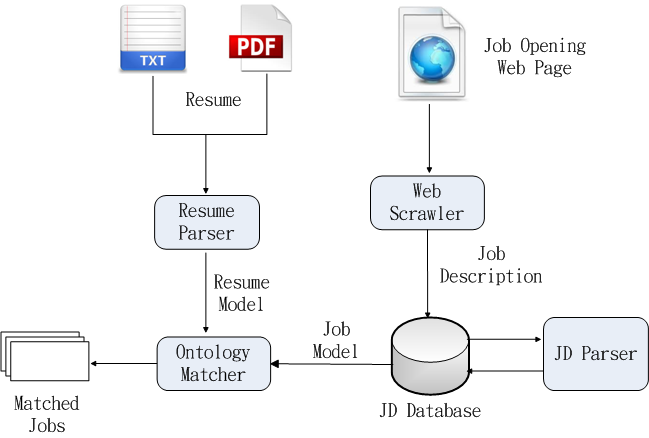
\includegraphics[scale=0.5]{images/arch.png}
  \caption{System Architecture}
  \label{fig:arch}
\end{figure}

\section{Text Processing Stages}

Information Extraction is the task of automatically extracting structured information such as entities, relationships between entities, and attributes describing entities from unstructured sources~\cite{sarawagi2008information}. The IE framework in our system uses six stages in order to extract the information from job descriptions: HTML parsing, segmenting, preprocessing, tokenizing, labeling and pattern matching, which is show in Figure~\ref{fig:Pipeline}.

1) The \textbf{HTML Parsing} will parse the web pages that contain job descriptions, which are obtained from web crawler. The parser uses HTML tag template to extract attributes of the jobs, like job title, location, company name, content and so on. A job will be saved as a record with these attributes in the database. In the record, the content field contains the text part of the job description, which will be processed in later stages.

2) In the \textbf{segmenting stage}, the content field of the job description is be separated into paragraphs according HTML tags. Then paragraphs are separated into sentences by either HTML tags or punctuation, and after this step, all HTML tags will be removed.

3) Web pages of job description are created in different character sets, (e.g. UTF8 and ISO 8859-1), and almost always contain some unreadable characters. In the \textbf{prepossessing stage}, characters in the sentences are converted to ASCII characters, unreadable characters will be deleted, and some punctuation will be replaced by spaces (e.g. / and -).

4) In the \textbf{tokenizing stage}, the sentences will be tokenized into arrays of tokens by NLTK~\cite{bird2006nltk}.

5) In the \textbf{labeling stage}, the sentences will be given two layers of labels by a dictionary matching approach. The labels in the first layer are the semantic value of the text, and the labels in the second layer are the ontology hypernym of the labels in the first layers.

6) In the \textbf{pattern matching} stage, the FST library is used to matching the labels of the labeled sentences.  If a layered sentence match any pre-defined pattern, the information will be extracted and added to the job model. After every sentence of a job description has be processed, a job model will be created and saved in the database. More details about matching will follow in Section C.

\begin{figure}[htbp]
  \centering
  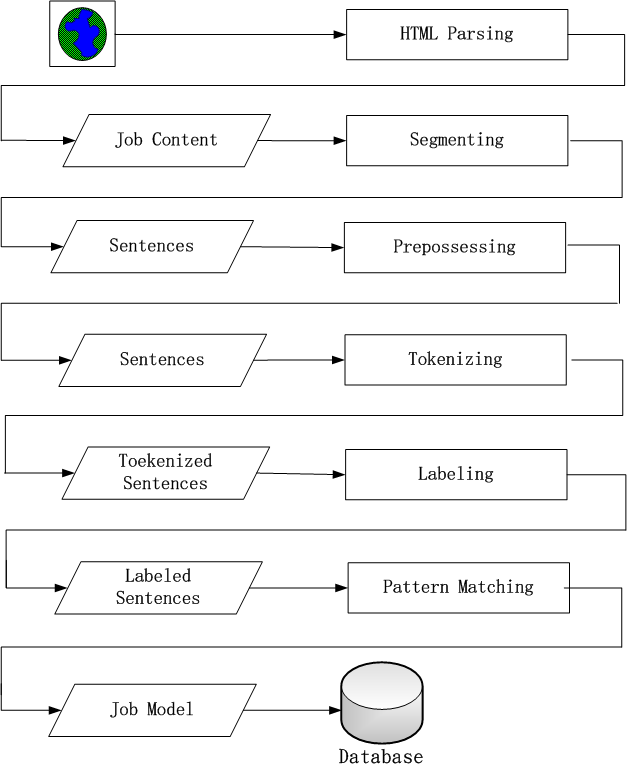
\includegraphics[scale=0.4]{images/pipeline2.png}
  \caption{Job Description Process Pipeline}
  \label{fig:Pipeline}
\end{figure}

\section{System Implementation}

We will describe some implementation details here. The whole system is implemented in Python and uses some third party libraries and frameworks. We used Flask, a lightweight web framework, to build the web application. We used Rdflib as the Web Ontology Language (OWL) file parser, Python Lex-Yacc (PLY) as the token regular expression compiler, whoosh as the inverted index builder and Beautiful Soup as the HTML parser.  All the jobs retrieved by the Web Crawler are stored in the MongoDB NoSQL database.  For the natural language processing procedure, we used Natural Language Toolkit (NLTK), a  natural language processing library, to extract and  tokenize the sentences.

\section{System Interface}

The system provides some interfaces to end users. The most important interfaces are the web pages like: reviewing all the jobs in the database, searching the jobs by keyword (Figure~\ref{fig:joblist}),  uploading users' r\'esum\'es (Figure~\ref{fig:upload_resume}),  matching the jobs with a r\'esum\'e (Figure~\ref{fig:match_resume}) and searching the jobs with both keyword and the r\'esum\'e (Figure~\ref{fig:keyword_resume}).

\begin{figure}[htbp]
  \centering
  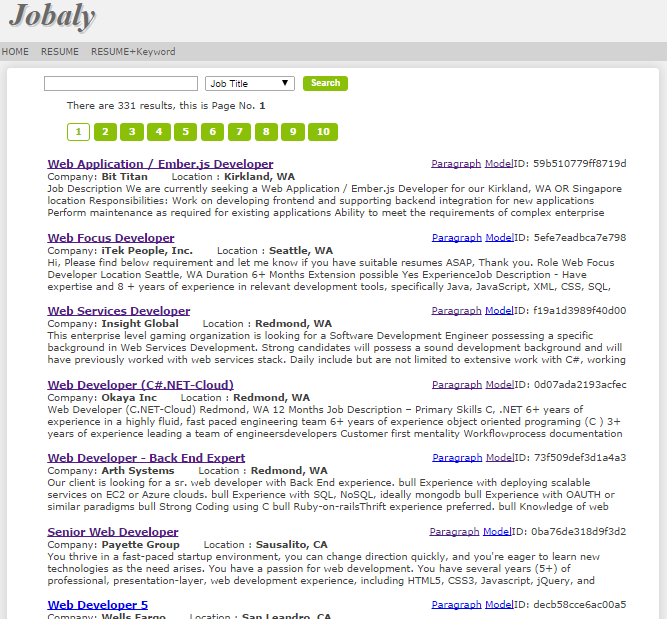
\includegraphics[scale=0.5]{images/joblist.png}
  \caption{Job Description List}
  \label{fig:joblist}
\end{figure}


\begin{figure}[htbp]
  \centering
  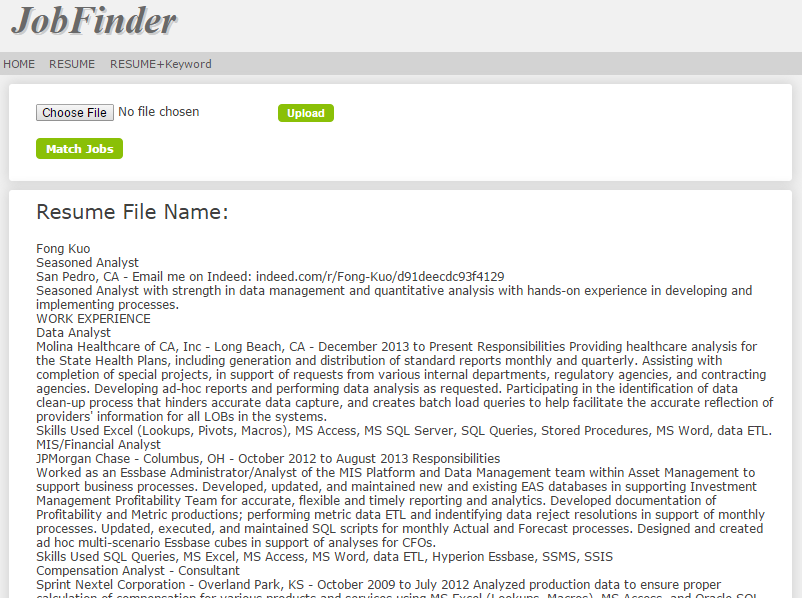
\includegraphics[scale=0.5]{images/upload_resume.png}
  \caption{Upload Resume}
  \label{fig:upload_resume}
\end{figure}

\begin{figure}[htbp]
  \centering
  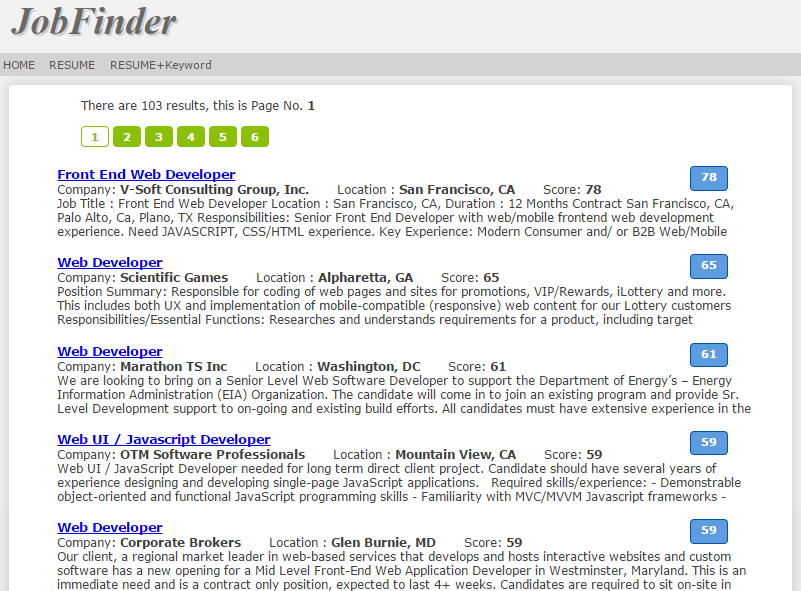
\includegraphics[scale=0.5]{images/match_resume.png}
  \caption{Resume Job matching }
  \label{fig:match_resume}
\end{figure}

\begin{figure}[htbp]
  \centering
  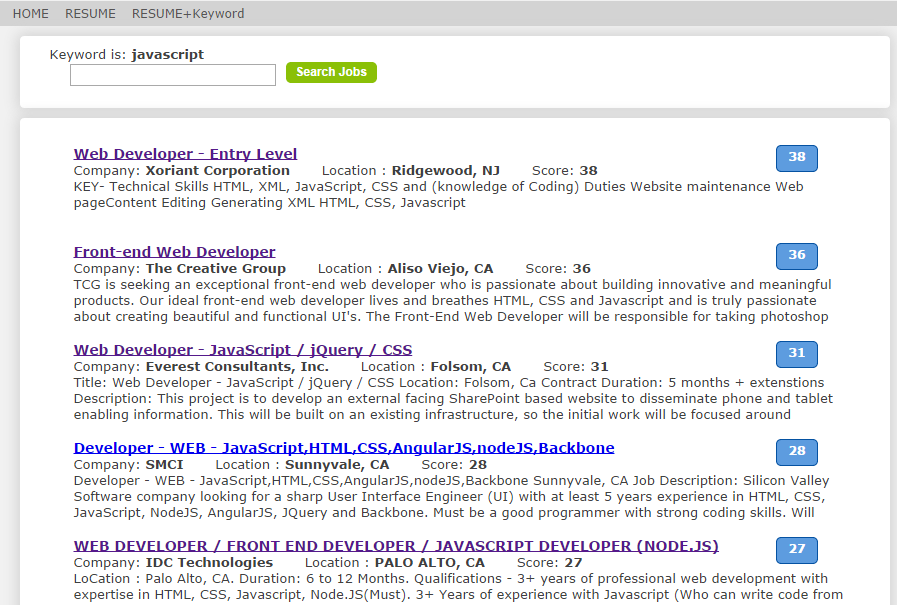
\includegraphics[scale=0.5]{images/keyword_resume.png}
  \caption{Combine the Keyword and Resume Matching}
  \label{fig:keyword_resume}
\end{figure}






